\section{Experiments}
\label{sec:experiments}
% \vspace{-0.1in}
We conduct comprehensive experiments to evaluate MetaFind across multiple dimensions, including object-level retrieval, scene-level layout-aware retrieval, and robustness under varying design choices. We begin by introducing our experimental setup, datasets, and baseline adaptations. We then present quantitative results on the Objaverse-LVIS dataset to assess retrieval performance under different modality combinations. Next, we evaluate scene-level quality on the ProcTHOR dataset, highlighting the benefits of layout-aware retrieval using our ESSGNN context encoder. We further perform extensive ablation studies to analyze the contribution of core architectural components and training strategies. Finally, we assess generalization across scene complexities and provide qualitative visualizations to showcase the real-world effectiveness of MetaFind.
% \vspace{-0.05in}
\subsection{Experimental Setup}
% \vspace{-0.05in}
\paragraph{Datasets} We evaluate MetaFind across both object-level and scene-level retrieval settings. The object-level experiments are conducted on the annotated Objaverse-LVIS dataset containing 48K unique 3D assets. For scene-level layout-aware retrieval, we use the ProcTHOR-10K dataset containing over 10,000 procedurally generated house layouts constructed from over 3,000 curated 3D assets. In both datasets, we allocate 80\% of the data for training and reserve the remaining 20\% for testing. While our experiments currently use single-room indoor scenes, the framework is designed to generalize to open-world settings; the $\mathrm{SE}(3)$-equivariant design specifically targets robustness to large-scale and dynamic environments.
% \vspace{-0.05in}
\paragraph{Baselines} 
\textbf{ULIP}~\cite{xue2024ulip} is a tri-modal single-tower model that aligns text, image, and point cloud modalities into a unified embedding space through joint representation learning. \textbf{OpenShape}~\cite{liu2023openshape} adopts a dual-tower contrastive retrieval design, supporting text-to-3D and image-to-3D retrieval via large-scale vision-language pretraining. \textbf{SCA3D}~\cite{ren2025sca3d} focuses on point cloud-text retrieval and improves robustness using self-augmented contrastive learning, though it lacks multi-modal query fusion capabilities. 
% \textbf{COM3D}~\cite{wu2024com3d} is a compositional retrieval model that incorporates spatial priors and semantic cues for improved category-level 3D asset retrieval from textual input. 
\textbf{Uni3DL}~\cite{li2023uni3dl} and \textbf{Uni3D}~\cite{zhou2023uni3d} present unified architectures for 3D-language-image understanding, supporting multiple modalities inputs. Finally, \textbf{OmniBind}~\cite{wang2024omnibindlargescaleomnimultimodal} offers a scalable omni-modality representation space that supports combinations of text, image, audio, and point cloud inputs, though it is not optimized for layout-aware or scene-conditioned retrieval.

Since most existing retrieval models (e.g., ULIP, OpenShape) are not designed to handle arbitrary combinations of input modalities, we limit our baselines to pre-trained single-tower encoders that support at least one of the three modalities: text, image, and point cloud. To create a fair comparison within a dual-tower retrieval paradigm, we extend each baseline by adding a simple \textit{mean pooling layer} to aggregate available modalities, and use these fused embeddings to retrieve from a pre-encoded gallery. For completeness, we also include our own dual-tower model with a mean fusion layer but without layout context as a direct ablation baseline. The temperature is 0.5 for all experiments.

% \vspace{-0.05in}
\paragraph{Metrics} We benchmark MetaFind and all variants using standard retrieval metrics, including top-$k$ retrieval accuracy (R@1, R@5). To assess scene-level performance, we further evaluate the compositional quality of generated scenes along two axes: structural coherence and stylistic consistency. These aspects are quantitatively scored using a GPT-4o-based aesthetic and alignment evaluator, and qualitatively validated through human preference studies conducted on a subset of generated scenes. This dual evaluation setup provides a comprehensive assessment of both retrieval accuracy and real-world usability in downstream scene construction.


% \vspace{-0.05in}
\subsection{Retrieval Performance on Objaverse-LVIS}
% \vspace{-0.05in}
We first evaluate the object-level retrieval performance on the annotated Objaverse-LVIS dataset, which comprises 48K high-quality 3D assets with structured textual descriptions and multi-view image renders. This evaluation focuses on the core capability of MetaFind to support flexible, modality-compositional retrieval, especially under partial modality conditions. All methods are evaluated under seven query conditions: text-only, image-only, point cloud-only, text+image, text+point cloud, image+point cloud, and full (text+image+point cloud). As shown in Table~\ref{tab:objaverse-results}, MetaFind without ESSGNN outperforms all baseline models across different settings. Notably, since other models do not adopt a dual-tower design, their "PC only" performance reflects retrieval using identical embeddings for both query and gallery, leading to inflated accuracy. In contrast, our dual-tower framework introduces more cross-modality retrieval, which results in lower accuracy under the "PC only". Nevertheless, MetaFind demonstrates stronger performance under partial modality conditions, highlighting its capability in multimodal fusion. After integrating the ESSGNN, while the overall scene quality is improved, we observe a drop in accuracy due to the added encoded information. This reflects a temporary and explainable trade-off between object-level precision and scene-level coherence. Stage-1 pretraining on Objaverse-LVIS uses isolated assets (no layout) and no ESSGNN; Stage-2 fine-tuning introduces ESSGNN on ProcTHOR (layout-rich, different asset distribution). Although the retrieval objective is unchanged, the fusion layer becomes partially adapted to layout-conditioned features, creating a feature-attribution mismatch when evaluating on Objaverse-LVIS (which lacks layout and disables ESSGNN). A practical mitigation is to maintain two fusion heads: a layout-free head (Stage-1) and a scene-aware head (Stage-2), selected at inference by context availability. Using the Stage-1 head reproduces the “w/o ESSGNN” numbers (omitted for brevity). In our reported results, we instead explore a single shared head by freezing both encoders in Stage-2, updating only ESSGNN and the fusion, and applying stochastic scene dropout (30\%) to expose the model to layout-free inputs; some accuracy loss remains due to residual attribution drift.

\begin{table}[h]
\centering
% \vspace{-0.2in}
\caption{Retrieval accuracy (R@1 / R@5) on Objaverse-LVIS under different query modality combinations. MetaFind consistently outperforms all baselines across both complete and incomplete query settings. `--` indicates that the method does not support the corresponding modality combination.}
\label{tab:objaverse-results}
\resizebox{\textwidth}{!}{%
\begin{tabular}{lccccccc}
\toprule
\textbf{Method} & \textbf{Text Only} & \textbf{Image Only} & \textbf{PC Only} & \textbf{T + I} & \textbf{T + PC} & \textbf{I + PC} & \textbf{T + I + PC} \\
\midrule
ULIP~\cite{xue2024ulip} & 0.1 / 0.9 & 0.1 / 1.3 & 97.9 / 99.4 & 0 / 0.3  & 33.9 / 58 & 22.6 / 41.6 & 6.4 / 15.9 \\
OpenShape~\cite{liu2023openshape} &  0.6 / 1.7 & 0.3 / 1.1 & 98.4 / 99.7 & 0 / 0.5 & 35.1 / 61.4 & 25.0 / 44.3 & 7.0 / 17.2 \\
SCA3D~\cite{ren2025sca3d} & 6.9 / 10.4 & -- & 98.1 / 99.3 & -- & 39.7 / 65.2 & -- & -- \\
% COM3D~\cite{wu2024com3d} & X / X & X / X & X / X & X / X & X / X & X / X & X / X \\
Uni3DL~\cite{li2023uni3dl} & 4.5 / 9.2 & -- & \underline{98.5} / \textbf{99.8} & -- & 37.4 / 63.9 & -- & -- \\
Uni3D~\cite{zhou2023uni3d} & 1.7 / 3.9 & 1.2 / 2.5 & 98.3 / 99.4 & 0.5 / 1.1 & 36.3 / 63.6 & 26.1 / 44.8 & 8.2 / 19.1 \\
OmniBind (Base) & 1.2 / 2.8 & 0.6 / 1.4 & 98.3 / 99.6 & 0 / 0.4 & 34.0 / 55.9 & 21.5 / 38.7 & 5.5 / 13.8 \\
OmniBind (Large) & 2.7 / 4.0 & 0.9 / 1.8 & 98.2 / 99.3 & 0.1 / 0.4 & 35.2 / 56.7 & 23.4 / 40.9 & 6.0 / 16.7 \\
OmniBind (Full)\cite{wang2024omnibindlargescaleomnimultimodal} & 5.3 / 11.7 & 2.3 / 3.5 & \textbf{99.0} / \underline{99.7} & 0.5 / 1.2 & 37.5 / 60.8 & 27.5 / 46.4 & 11.9 / 23.4 \\
MetaFind w/o ESSGNN & \textbf{13.8 / 23.1} & \textbf{11.7 / 19.2} & 75.1 / 78.0 & \textbf{17.2 / 21.8} & \textbf{44.5 / 71.3} & \textbf{45.8 / 73.1} & \textbf{51.7 / 76.5} \\
MetaFind w/ ESSGNN & \underline{11.3 / 21.5} &  \underline{10.5 / 15.9}  & 63.2 / 66.5 & \underline{15.9 / 20.3} & \underline{41.2 / 68.8} & \underline{42.0 / 70.4} & \underline{48.2 / 74.9}\\ 
\bottomrule
\end{tabular}%
}
% \vspace{-0.15in}
\end{table}
% \vspace{-0.05in}
\subsection{Scene-Level Retrieval with Layout Context}
% \vspace{-0.05in}
To evaluate the benefit of layout-aware retrieval in realistic scenes, we assess MetaFind on a scene generation pipeline of I-Design \cite{ccelen2024design}. It can generate a 3D scene with a given room description by designing, retrieving, and arranging.  In the original paper, they use OpenShape\cite{liu2023openshape} to retrieve the objects. Here, we compare the performance of MetaFind with and without the ESSGNN layout encoder. No retrieval accuracy, we assess the overall quality of composed scenes using both automated and human evaluations across four key dimensions: (1) Overall Aesthetic and Atmosphere: Measures the visual appeal and mood of the composed scene; (2) Color Scheme and Material Choices: Evaluates consistency in textures, colors, and materials between newly retrieved assets and the existing scene; (3) Scene Coherence: Assesses how well the inserted assets align with the scene's spatial and semantic context; and (4) Realism and 3D Geometric Consistency: Checks for physically plausible placements, avoiding collisions or unnatural geometry. Each dimension is rated on a scale from 1 (poor) to 5 (excellent), independently by GPT-4o and five expert human annotators on a set of 200 randomly sampled scenes. For GPT-4o, we provide scene layouts and rendered views, with prompts aligned to the respective evaluation criteria. Final scores are averaged across annotators and samples.

\begin{table}[h]
\centering
% \vspace{-0.15in}
\caption{Scene-level quality comparison across four evaluation dimensions. MetaFind (with GSSNN) achieves the highest scores across both GPT-4o and human evaluations, demonstrating superior spatial coherence and aesthetic quality in composed scenes.}
\label{tab:layout-results}
\resizebox{\textwidth}{!}{%
\begin{tabular}{lcccccccc}
\toprule
\multirow{2}{*}{\textbf{Method}} & \multicolumn{2}{c}{\textbf{Aesthetic}} & \multicolumn{2}{c}{\textbf{Color \& Material}} & \multicolumn{2}{c}{\textbf{Scene Coherence}} & \multicolumn{2}{c}{\textbf{Realism \& Geometry}} \\
\cmidrule(lr){2-3} \cmidrule(lr){4-5} \cmidrule(lr){6-7} \cmidrule(lr){8-9}
 & GPT-4o & Human & GPT-4o & Human & GPT-4o & Human & GPT-4o & Human \\
\midrule
ULIP~\cite{xue2024ulip} & 2.91 & 3.02 & 2.84 & 2.97 & 2.76 & 2.89 & 2.70 & 2.81 \\
OpenShape~\cite{liu2023openshape} & 3.14 & 3.28 & 3.08 & 3.19 & 3.01 & 3.11 & 2.95 & 3.06 \\
MetaFind w/o ESSGNN & \underline{3.42} & \underline{3.55} & \underline{3.31} & \underline{3.41} & \underline{3.26} & \underline{3.33} & \underline{3.22} & \underline{3.30} \\
MetaFind w/ ESSGNN & \textbf{4.13} & \textbf{4.25} & \textbf{4.04} & \textbf{4.17} & \textbf{4.10} & \textbf{4.21} & \textbf{4.06} & \textbf{4.18} \\
\bottomrule
\end{tabular}
}
% \vspace{-0.1in}
\end{table}
Figures~\ref{fig:essgnn_row4}, \ref{fig:essgnn_comparison} show qualitative comparisons of scene generation with and without the ESSGNN encoder. The first example is a classical-style lounge, which, without ESSGNN, suffers from inconsistent object styles and poor layout organization. With ESSGNN, the scene is more coherent, with well-aligned furniture and logical arrangement for group interaction. The second example is an aged archive room. Without ESSGNN, the objects appear mismatched, while the ESSGNN-generated version offers a more functional and visually consistent space, with well-placed furniture suitable for a reading environment. These results demonstrate that ESSGNN improves both stylistic consistency and layout functionality. This qualitative improvement is also reflected in the quantitative results shown in Table~\ref{tab:layout-results}, where MetaFind with ESSGNN achieves the highest scores across all evaluation metrics. In particular, the gains in scene coherence and realism highlight the encoder’s ability to model spatial relationships and stylistic alignment effectively. Together, these findings confirm the effectiveness of ESSGNN in generating high-quality, semantically grounded 3D scenes.


% \vspace{-0.05in}
\subsection{Ablation Studies}
% \vspace{-0.05in}
\begin{table}[h]
\centering
% \vspace{-0.1in}
\caption{Ablation study (Text Only). We report top-1 retrieval accuracy (R@1) on the Object-level task, GPT-4o-based aesthetic score, and scene-level coherence score on the Scene-Level task.}
\label{tab:ablation}
\resizebox{\textwidth}{!}{
\begin{tabular}{lccc}
\toprule
\textbf{Variant} & \textbf{R@1 (\%)} & \textbf{Aesthetic (GPT-4o)} & \textbf{Scene Coherence (GPT-4o)} \\
\midrule
\textbf{MetaFind (Full, bidirectional) w/ iterative retrieval \& ESSGNN} & 11.4 & \textbf{4.1} & \textbf{4.2} \\
\midrule
w/o iterative retrieval & 11.3 & \underline{4.0} & \underline{4.1} \\
w/o Layout Context & \textbf{13.5} & 3.4 & 3.3 \\
w/ Layout Context (GAT) & 11.0 & 3.4 & 3.7 \\
\midrule
Fusion = Mean & 9.4 & 3.2 & 3.5 \\
Fusion = MLPs & 9.9 & 3.3 & 3.5 \\
\midrule
Modality Dropout = 10\% & 7.3 & 3.4 & 3.5 \\
Modality Dropout = 50\% & \underline{13.2} & 3.1 & 3.2 \\
\midrule
Train fuser only & 8.7 & 3.3 & 3.2 \\
\midrule
Padding missing modalities with 0& 10.5 & 3.1 & 3.1 \\
\bottomrule
\end{tabular}
}
% \vspace{-0.1in}
\end{table}

\begin{figure*}[t]
  \centering
  \begin{subfigure}[b]{0.23\textwidth}
    \centering
    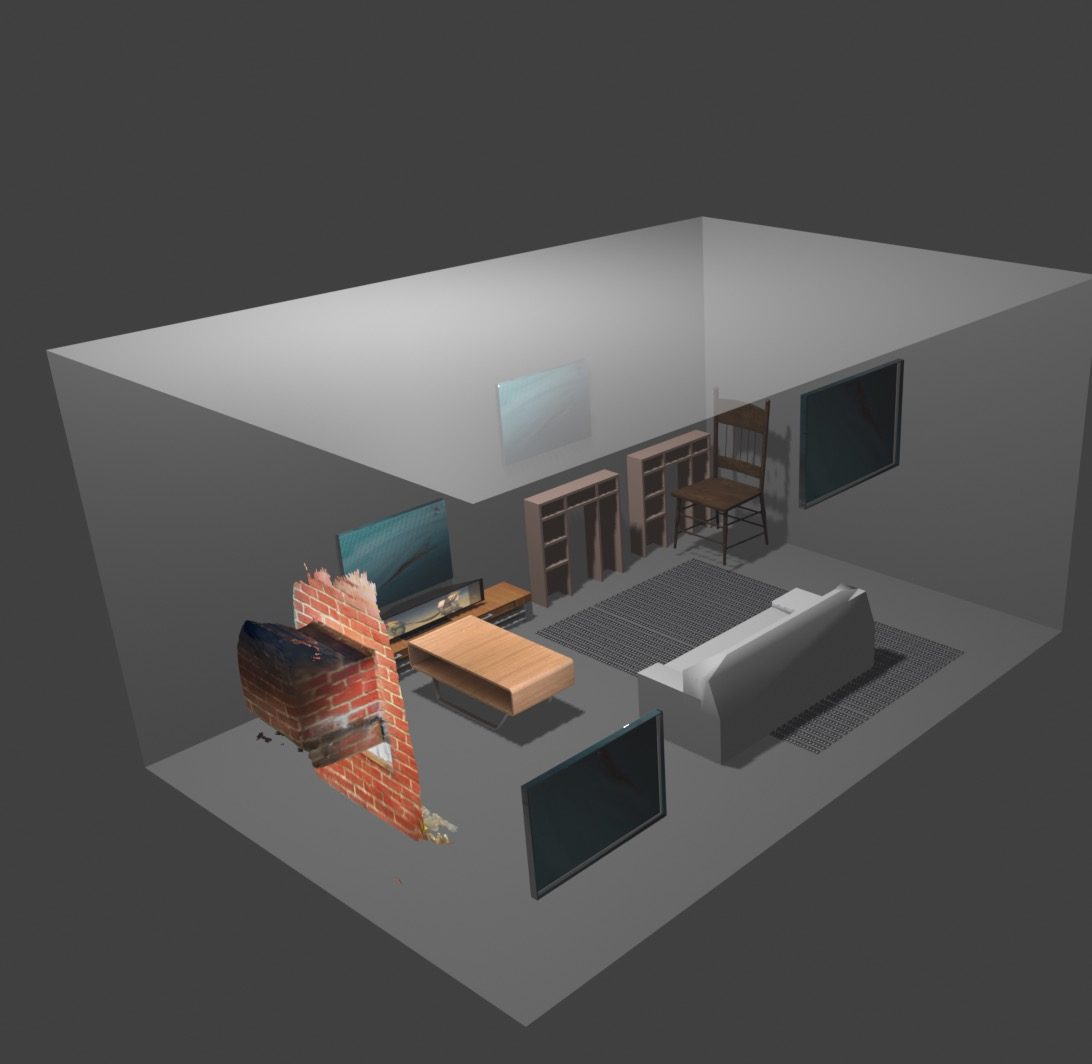
\includegraphics[width=3.5cm, height=3.5cm]{scene1_no_essgnn.png}
    \caption*{Room 1\\Without ESSGNN}
  \end{subfigure}
  \begin{subfigure}[b]{0.23\textwidth}
    \centering
    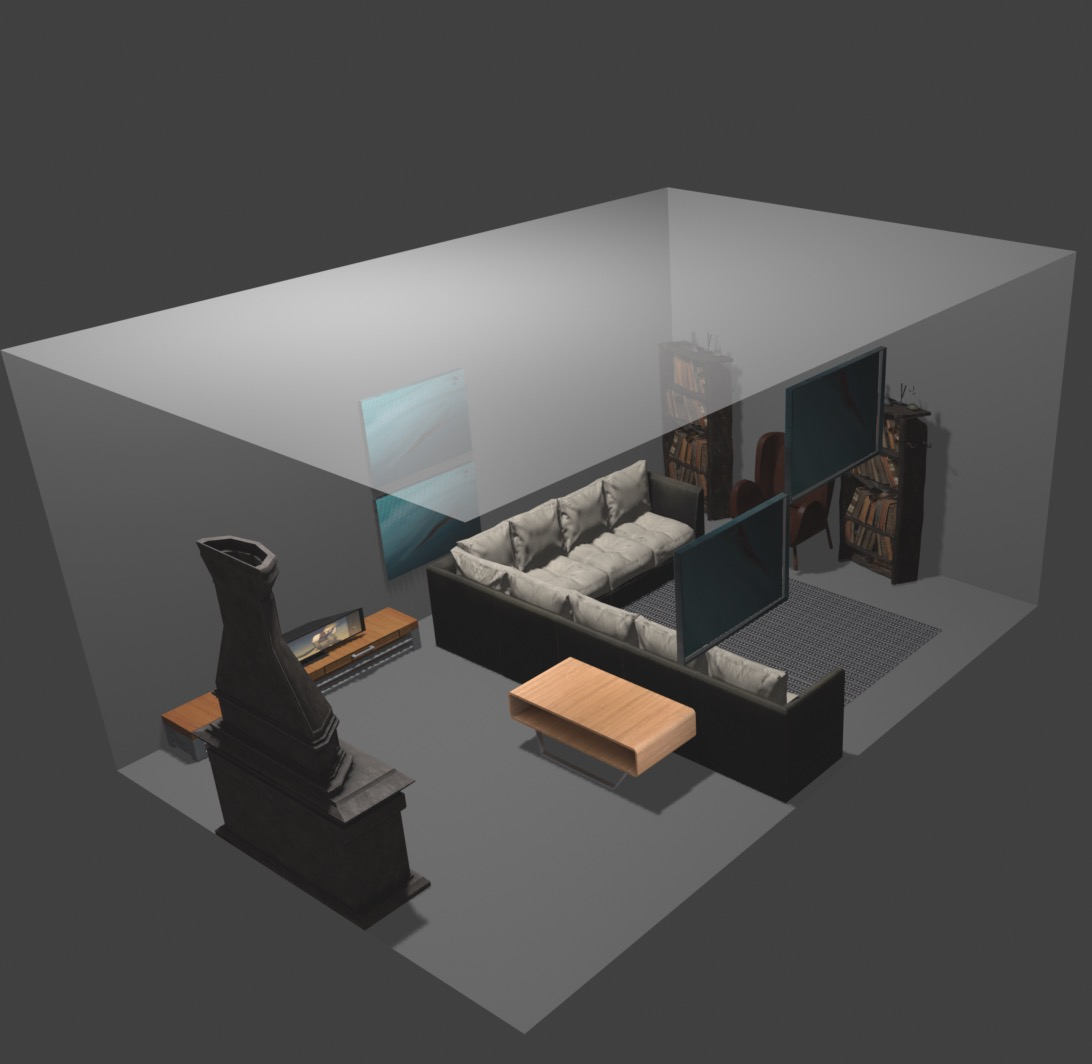
\includegraphics[width=3.5cm, height=3.5cm]{scene1_with_essgnn.png}
    \caption*{Room 1\\With ESSGNN}
  \end{subfigure}
  \begin{subfigure}[b]{0.23\textwidth}
    \centering
    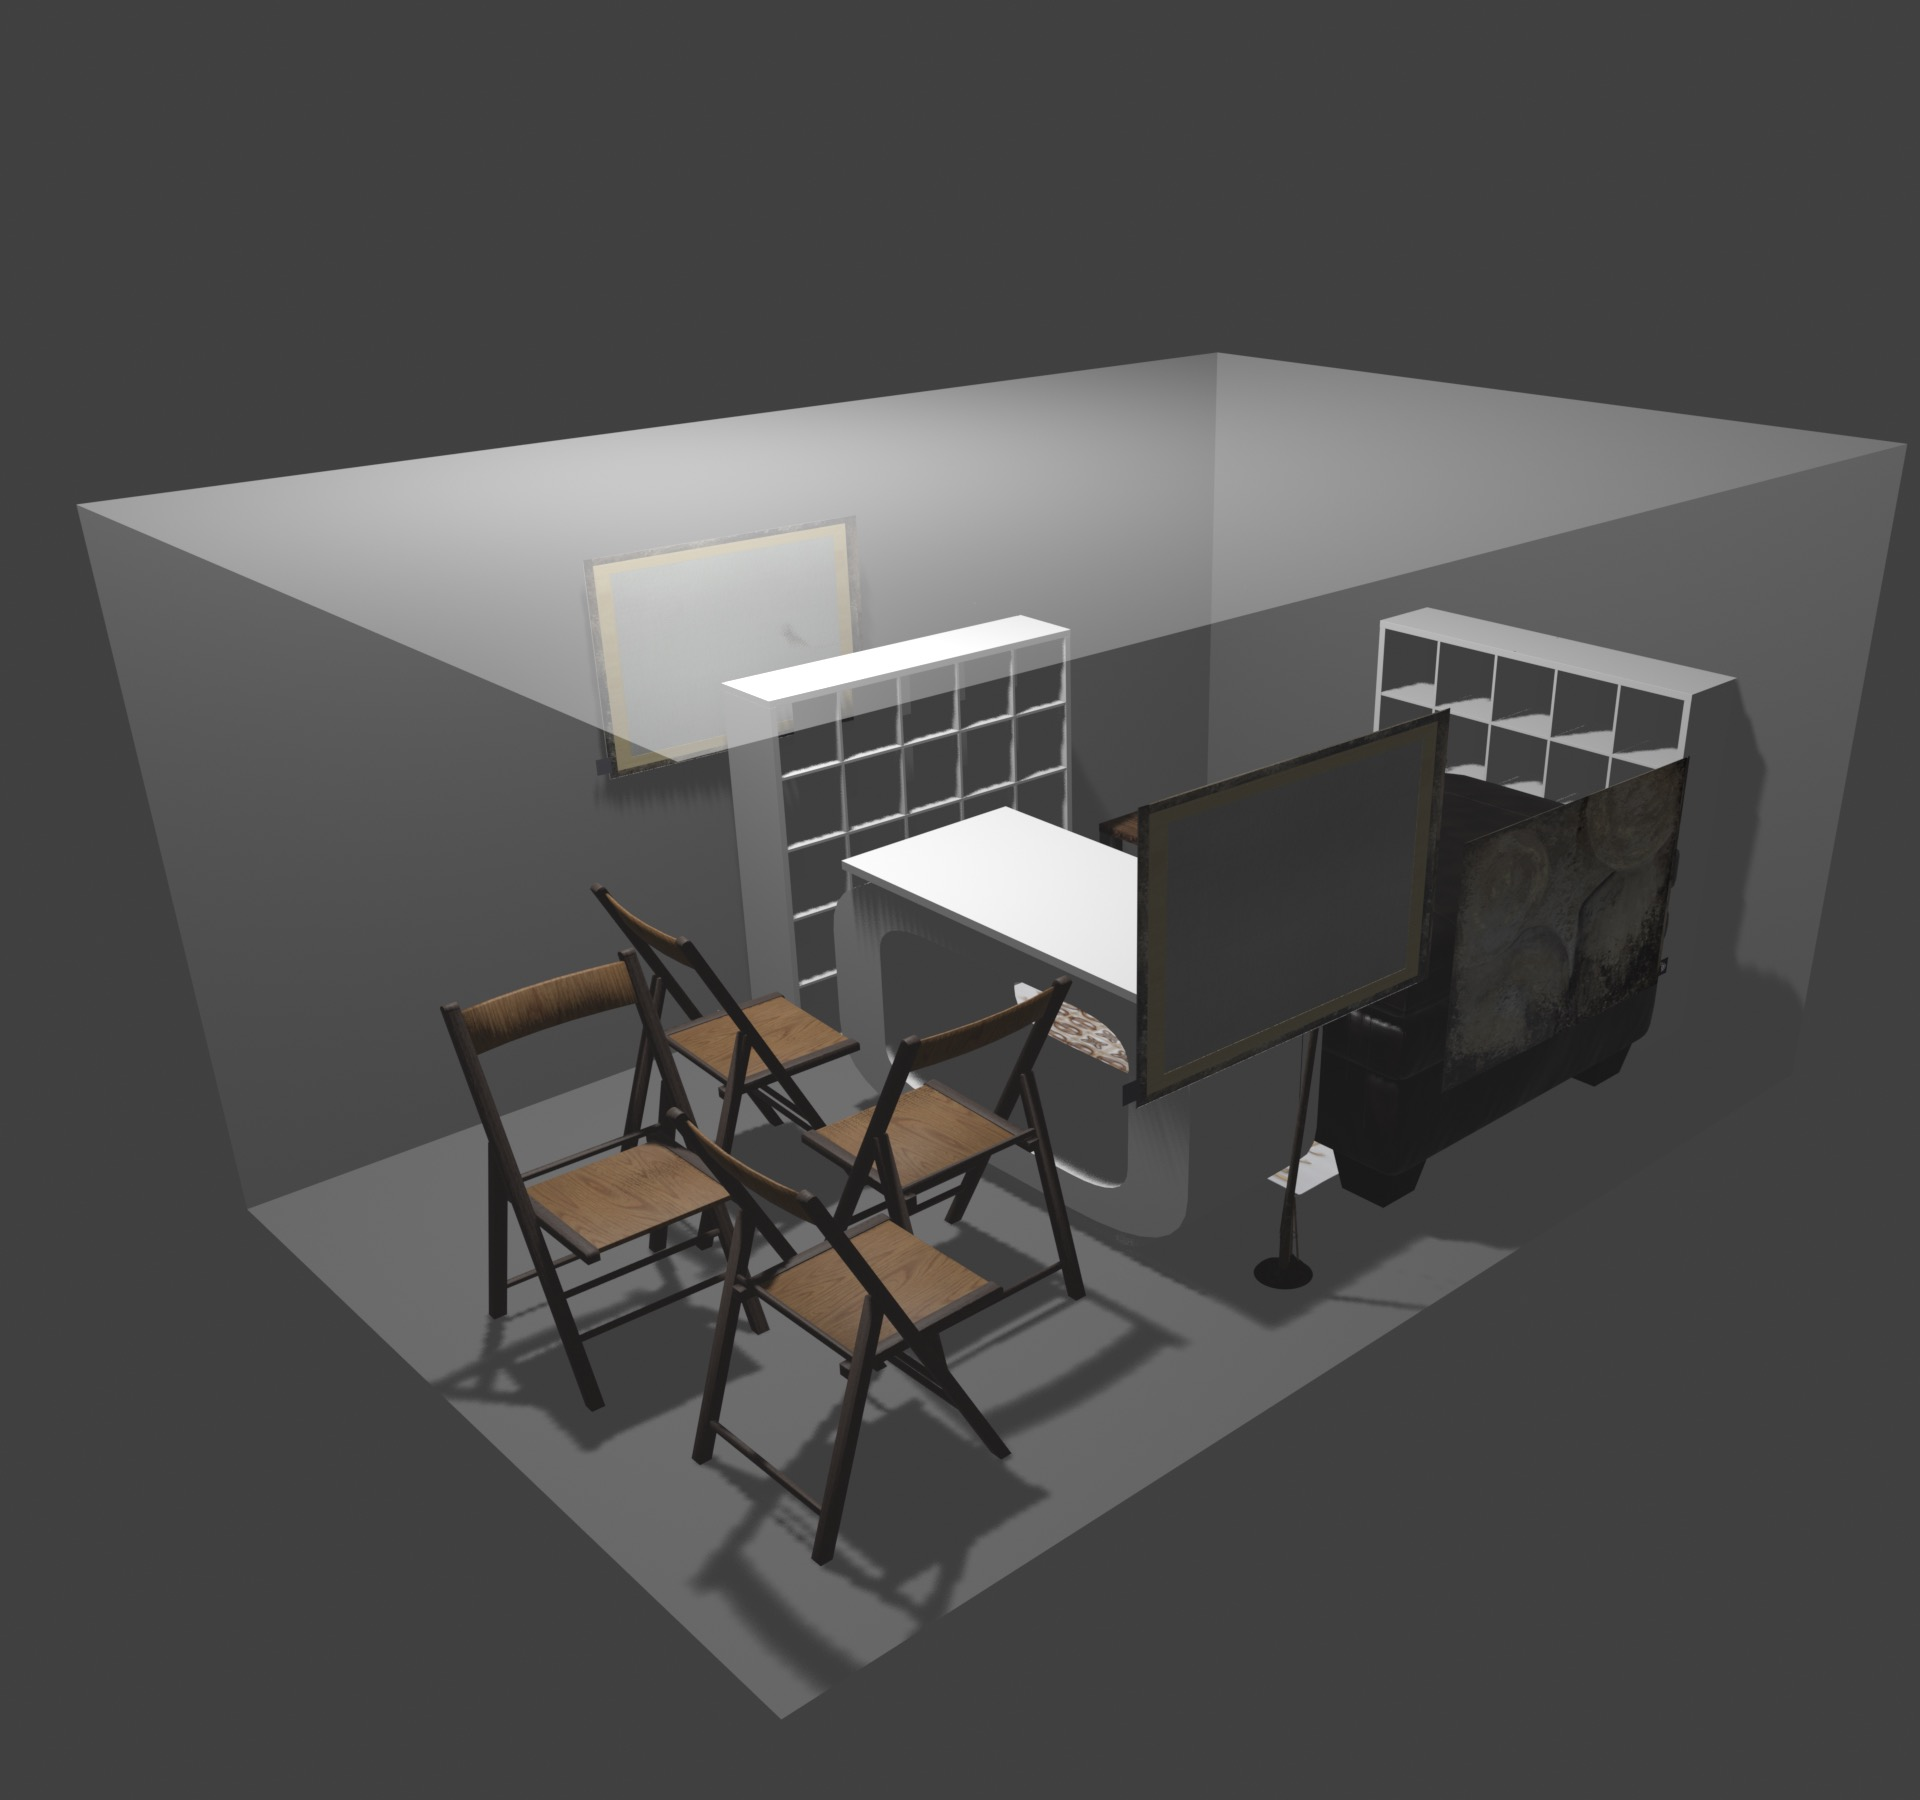
\includegraphics[width=3.5cm, height=3.5cm]{scene2_no_essgnn.png}
    \caption*{Room 2\\Without ESSGNN}
  \end{subfigure}
  \begin{subfigure}[b]{0.23\textwidth}
    \centering
    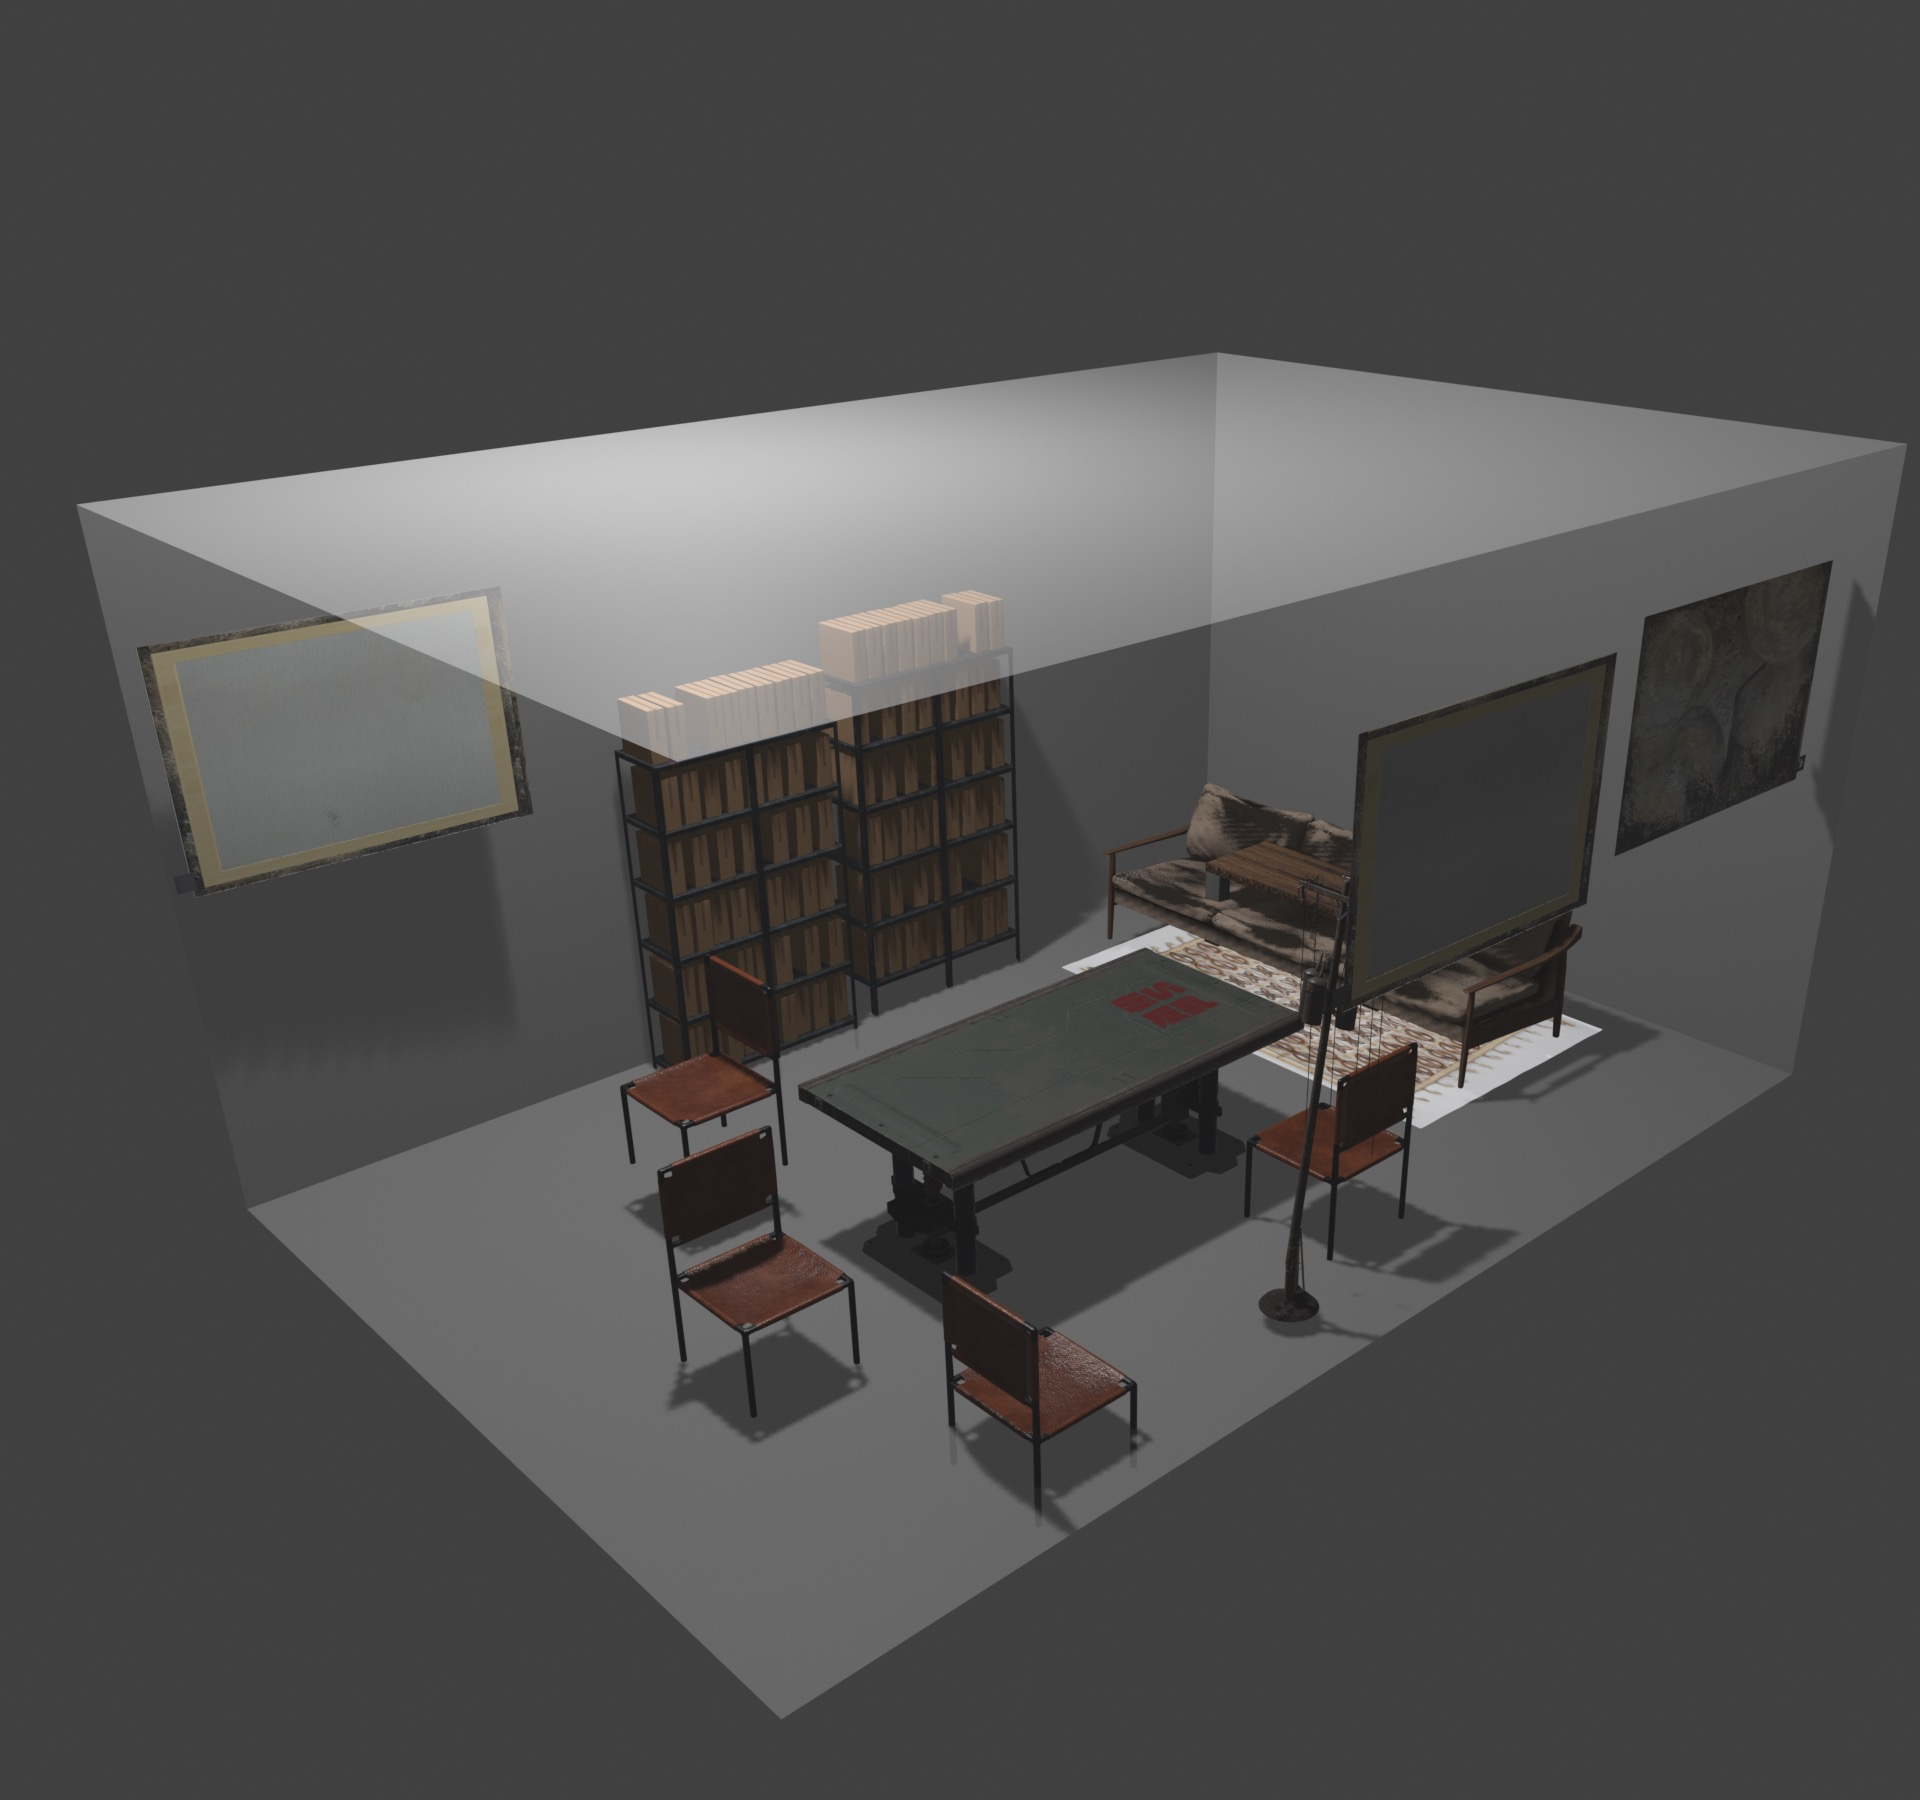
\includegraphics[width=3.5cm, height=3.5cm]{scene2_with_essgnn.png}
    \caption*{Room 2\\With ESSGNN}
  \end{subfigure}

  \caption{Visual comparison of scene generation with and without the ESSGNN encoder across two room descriptions. Room 1 — "A classical-style lounge for group leisure and conversation"; Room 2 — “An aged archive room for research and consultation”}
  \label{fig:essgnn_row4}
  % \vspace{-0.15in}
\end{figure*}

We conduct ablation studies to evaluate the effectiveness of key architectural components and training strategies in MetaFind, focusing on six dimensions: layout encoding, modality fusion strategies, modality dropout robustness, fusion granularity, gallery encoder flexibility, and missing modality handling. First, removing the ESSGNN layout encoder results in drops in scene realism, underscoring the critical role of spatial context. Regarding fusion strategies, while simple mean pooling offers computational efficiency, MLP and the final selected Transformer outperform others under partial modality conditions by dynamically reweighting available inputs. We also examine modality dropout rates during training, finding that a 30\% rate strikes the best balance between robustness and accuracy. Lower rates lead to overfitting on full-modality inputs, whereas higher rates introduce instability. Additionally, we compare fusion granularity strategies, revealing that while training only the fusion module in the query encoder improves efficiency, full encoder fine-tuning yields better performance by allowing earlier layers to adapt to modality-aware supervision. Finally, in handling missing modalities, modality masking outperforms zero-padding by preventing zero embedding interference and promoting robustness through sparsity-aware fusion. Results across these ablations, summarized in Table~\ref{tab:ablation}, demonstrate the modularity and resilience of MetaFind under diverse design choices.
